\documentclass{article}
\usepackage[utf8]{inputenc}
\usepackage{mathtools, amssymb, amsthm}
\usepackage{fullpage}
\usepackage{physics}
\usepackage{siunitx}
\usepackage{comment}

\usepackage{tikz}
\usetikzlibrary{arrows}

\usepackage[
    pdfusetitle,
    colorlinks
]{hyperref}

\title{Modeling and simulation of the SLM process}
\date{\today}
\author{Oleg Rogozin}

\newcommand{\dder}[2][]{\Delta_{#2}#1}
\newcommand{\diag}[1]{\qty(#1)^\mathrm{diag}}
\newcommand{\fusion}[1]{{#1}^\mathrm{fus}}

\begin{document}
\maketitle
\tableofcontents

\section{Formulation of the problem}

%%% The first law of thermodynamics
The conservation of energy for a substance at rest is described by the \(D\)-dimensional heat-conduction equation
\begin{equation}\label{eq:heat_conduction}
	\rho\pdv{h(T)}{t} = \pdv{x_i}\qty( k(\psi,T)\pdv{T}{x_i} ),
\end{equation}
where \(x_i\) are the physical coordinates (\si{m}), \(t\) is the time (\si{s}),
\(\rho\) is the density (\si{kg/m}\(^D\)), \(h\) is the specific enthalpy (\si{J/kg}),
\(T\) is the temperature (\si{\K}), \(k\) is the thermal conductivity (\si{W/Km}\(^{D-2}\)),
\(\psi\) is the porosity. Let
\begin{equation}\label{eq:porosity_variables}
	\rho = \rho_0(1-\psi_0), \quad k = k_0(T)(1-\psi),
\end{equation}
where \(\rho_0\) and \(k_0\) is the density and thermal conductivity of the bulk material, respectively,
\(\psi_0\) is the initial porosity.

%%% Introduce a liquid fraction
To incorporate the fusion process into the model, let the enthalpy depends on the temperature as follows:
\begin{equation}\label{eq:enthalpy}
	h = \int_{T_0}^T c_p(\xi)\dd{\xi} + \fusion{h}\phi(h),
\end{equation}
where \(c_p\) is the specific heat capacity (\si{J/kgK}), \(\fusion{h}\) is the specific enthalpy of fusion (\si{J/kg}),
\(\phi\) is the liquid fraction (\(0 \leq \phi \leq 1\)).
\(\phi=0\) and \(\phi=1\) corresponds to the solid and liquid states, respectively.
Substituting~\eqref{eq:porosity_variables} and~\eqref{eq:enthalpy} into~\eqref{eq:heat_conduction}, we obtain
\begin{equation}\label{eq:heat_conduction2}
	\rho_0\pdv{h}{t} = \pdv{x_i}\qty( \frac{1-\psi}{1-\psi_0} \frac{k_0(T)}{c_p(T)}\pdv{h_*}{x_i} ),
\end{equation}
where \(h_* = h - \fusion{h}\phi\) is introduced for convenience.

%%% Change in thermophysical properties resulting from fusion process
The phase transition results in an abrupt change in the thermophysical properties \(f=c_p,k_0\) of the material;
therefore, they can be expressed as
\begin{equation}\label{eq:fusion_change}
	f = f_S(T) + \qty( f_L(T) - f_S(T) )\phi,
\end{equation}
where \(f_S\) and \(f_L\) correspond to solid and liquid properties.
The porosity change is irreversible in time:
\begin{equation}\label{eq:porosity}
	\psi(t) = \psi_0\min_{0\leq\tau\leq t}\qty( 1-\phi(h(\tau)) ).
\end{equation}

%%% Initial and boundary conditions
Consider a half-space problem \(x_D<0\) with the following boundary condition at \(x_D=0\):
\begin{equation}\label{eq:bc}
	k(\psi,T)\pdv{T}{x_D} = \frac{A(\psi)P}{(\pi R^2)^{(D-1)/2}}\exp\qty( -\frac{(x_i-x_{Bi}(t))^2}{R^2} )
	    - \alpha(T-T_0) - \epsilon\sigma T^{D+1},
\end{equation}
where \(A\) is the absorptivity, \(P\) is the laser power (\si{W}), \(R\) is the radius of the laser beam (\si{m}),
\(x_{Bi}\) are the coordinates of its center (\si{m}), \(\alpha\) is the convective heat transfer coefficient (\si{W/Km}\(^{D-1}\)),
\(\epsilon\) is the emissivity, \(\sigma\) is the Stefan--Boltzmann constant (\si{W/K}\(^{D+1}\)\si{m}\(^{D-1}\)).
The initial condition is \(T=T_0\) at \(t=0\).

\subsection{Dimensionless expressions}

Introduce the following dimensionless variables:
\begin{equation}\label{eq:dimensionless}
    \begin{aligned}
        x_i &= \hat{x}_iR, & t &= \hat{t}t_0, & h &= \hat{h}c_p(T_0)\Delta{T}, & T - T_0 &= \hat{T}\Delta{T}, \\
        P &= \hat{P} k_0(T_0)\Delta{T}R^{D-2}, & \alpha &= \hat{\alpha}\frac{k_0(T_0)}R, &
            \sigma &= \hat{\sigma}\frac{k_0(T_0)}{R\Delta{T}^D}, & T_0 &= \hat{T}_0\Delta{T}, \\
    \end{aligned}
\end{equation}
where \(t_0 = \rho_0 c_p(T_0) R^2/k_0(T_0)\) is the diffusive time scale at \(T=T_0\),
\(\Delta{T} = (T_S+T_L)/2 - T_0\) is the unit temperature,
\(T_S\) and \(T_L\) are the solidus and liquidus temperatures, respectively.
If \(|\pdv*{x_{Bi}}{t}|\) is of order \(U_0\), where \(U_0\) is the reference scanning speed (\si{m/s}),
then \(R/U_0\) is the convective time scale. Also denote
\begin{equation}\label{eq:dimensionless2}
    \hat{c}_p(\hat{T}) = \frac{c_p(T)}{c_p(T_0)}, \quad
    \hat{k}_0(\hat{T}) = \frac{k_0(T)}{k_0(T_0)}, \quad
    \hat{\phi}(\hat{h}) = \phi(h), \quad
    \hat{\psi}(\hat{h}) = \psi(h).
\end{equation}
Then~\eqref{eq:enthalpy},~\eqref{eq:heat_conduction2}, and~\eqref{eq:bc} take the following nondimensional form:
\begin{gather}
	\hat{h}_* \equiv \hat{h} - \fusion{\hat{h}}\hat{\phi} = \int_0^{\hat{T}} \hat{c}_p(\xi)\dd{\xi}, \label{eq:enthalpy_hats} \\
	\pdv{\hat{h}}{\hat{t}} = \pdv{\hat{x}_i}\qty(
	    \frac{1-\hat{\psi}}{1-\psi_0}
	    \frac{\hat{k}_0(\hat{T})}{\hat{c}_p(\hat{T})}\pdv{\hat{h}_*}{\hat{x}_i}
	), \label{eq:heat_conduction_hats} \\
	\qty(1 - \hat{\psi}) \frac{\hat{k}_0(\hat{T})}{\hat{c}_p(\hat{T})}\pdv{\hat{h}_*}{\hat{x}_D} +
	    \hat{\alpha}\hat{T} + \epsilon\hat{\sigma} \qty(\hat{T} + \hat{T}_0)^{D+1} =
	    \frac{A(\psi)\hat{P}}{\pi^{(D-1)/2}}\exp\qty( -\qty(\hat{x}_i-\hat{x}_{Bi}(t))^2 ). \label{eq:bc_hats}
\end{gather}
The initial condition is \(\hat{h} = 0\).

\subsection{Thermophysical properties}

For conventional materials, the required thermophysical properties can be reasonably approximated
by the three-parameter model (Fig.~\ref{fig:thermophysical})
\begin{equation}\label{eq:thermophysical_model}
	\hat{f} = 1 + \hat{f}'_S\hat{T} + \qty[
	    \fusion{\hat{f}} + \qty(\hat{f}'_L - \hat{f}'_S) \qty(\hat{T} - 1)
	]\hat{\phi},
\end{equation}
where \(\hat{f}'_{S,L}\) are the corresponding constant first temperature derivatives far from fusion process,
\(\fusion{\hat{f}}\) is the property jump at the phase transition.
Matching~\eqref{eq:thermophysical_model} with~\eqref{eq:fusion_change}, we obtain
\begin{equation}\label{eq:thermophysical_model_explicit}
	\hat{f}_S = 1 + \hat{f}'_S\hat{T}, \quad
	\hat{f}_L = \hat{f}_{L0} + \hat{f}'_L\hat{T},
\end{equation}
where \(\hat{f}_{L0} = 1 + \hat{f}'_S - \hat{f}'_L + \fusion{\hat{f}}\).

\begin{figure}
    \centering
    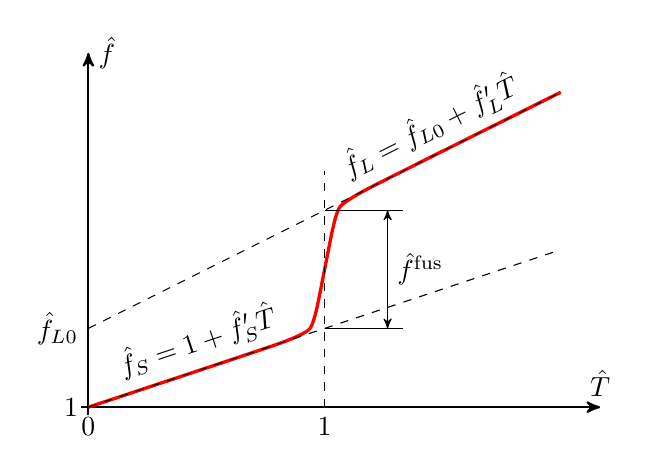
\begin{tikzpicture}[thick, >=stealth']
        \coordinate (O) at (0,0);
        \draw[->] (-0.1,0) -- (6.5,0) node[above] {$\hat{T}$} coordinate(xmax);
        \draw[->] (0,-0.1) -- (0,4.5) node[right] {$\hat{f}$} coordinate(ymax);

        \path (O) -- (3,1) node[midway,sloped,above] {$\hat{f}_S=1+\hat{f}'_S\hat{T}$}
            -- (3,2.5) -- (6,4) node[midway,sloped,above] {$\hat{f}_L=\hat{f}_{L0}+\hat{f}'_L\hat{T}$};
        \draw[red, very thick] plot[smooth,tension=0.3,mark=] coordinates{
            (0,0) (2.4,2.4/3) (2.8, 2.8/3+0.05) (2.9,3.5/2-0.5) (3.1,3.5/2+0.5) (3.2,2.5+0.2/2-0.05) (3.6,2.5+0.6/2) (6,4)};
        \draw[thin,dashed] (0,1) coordinate(A) -- (6,4);
        \draw[thin,dashed] (O) -- (6,2);
        \draw[thin,dashed] (3,0) coordinate(F) -- (3,3);

        \node[below] at (O) {$0$};
        \node[below] at (F) {$1$};
        \node[left] at (O) {$1$};
        \node[left] at (A) {$\hat{f}_{L0}$};

        \draw[thin] (3,1) -- (4,1);
        \draw[thin] (3,2.5) -- (4,2.5);
        \draw[thin,<->] (3.8,1) -- (3.8,2.5) node[midway,right] {$\fusion{\hat{f}}$};
    \end{tikzpicture}
    \caption{Dimensionless thermophysical properties versus temperature for the three-parameter model~\eqref{eq:thermophysical_model}.}
    \label{fig:thermophysical}
\end{figure}

\section{Liquid fraction models}

Impose the following physical requirements upon \(\hat\phi(\hat{h})\):
\begin{gather}
    0 \leq \dv{\hat\phi}{\hat{h}} \leq \eval{\dv{\hat\phi}{\hat{h}}}_{\hat{h}=\hat{h}(1)} =
        \frac1{\hat{h}(\hat{T}_L)-\hat{h}(\hat{T}_S)}, \label{eq:lf_monotonic}\\
    \hat\phi\qty(\hat{h}(1) - \hat{h}) = 1 - \hat\phi(\hat{h}) \quad \qty(\hat{h}\geq\hat{h}(1)), \label{eq:lf_symmetric}\\
    \begin{cases}
	\phi(\hat{h}) = \order{(\hat{h}(\hat{T}_S)-\hat{h})^{-\infty}} \quad \qty(\hat{h} < \hat{h}(\hat{T}_S)), \\
	    \phi(\hat{h}) = \order{(\hat{h}-\hat{h}(\hat{T}_L))^{-\infty}} \quad \qty(\hat{h} > \hat{h}(\hat{T}_L)).
	\end{cases}\label{eq:lf_exp_decay}
\end{gather}
Inequalities~\eqref{eq:lf_monotonic} are the monotonic condition and boundedness of the fusion rate,
\eqref{eq:lf_symmetric} is the symmetric property,
and~\eqref{eq:lf_exp_decay} describes an exponential decay of \(\hat\phi(\hat{h})\) outside the fusion range.

The simplest \(\mathcal{C}^0\) model for \(\hat{\phi}(\hat{h})\) can be constructed as a piecewise approximation
\begin{equation}\label{eq:lf_piecewise}
	\hat{\phi} = \begin{cases}
        0,                                           & \hat{h} \leq \hat{h}(\hat{T}_S), \\
        \frac{\hat{h}-\hat{h}(\hat{T}_S)}
            {\hat{h}(\hat{T}_L)-\hat{h}(\hat{T}_S)}, & \hat{h}(\hat{T}_S) < \hat{h} < \hat{h}(\hat{T}_L), \\
        1,                                           & \hat{h}(\hat{T}_L) \leq \hat{h}.
    \end{cases}
\end{equation}
Except \(\fusion{\hat{h}}\), \(\delta\fusion{\hat{T}} = \hat{T}_L - \hat{T}_S\)
is the only parameter of the fusion process  used in~\eqref{eq:lf_piecewise}.
Employing cubic splines near \(h_S\) and \(h_L\) yields the more realistic two-parameter \(\mathcal{C}^1\) model:
\begin{equation}\label{eq:lf_splines}
	\dots
\end{equation}

\section{Temperature evaluation}

For arbitrary \(\hat{\phi}(\hat{h})\), solution of~\eqref{eq:enthalpy_hats} is not straightforward.
However, the temperature is included in~\eqref{eq:heat_conduction_hats} only through thermophysical properties
and, therefore, can be evaluated quite roughly.
Direct dependence of boundary conditions~\eqref{eq:bc_hats} on temperature is also weak.
Several approaches can be proposed to find a simplified approximation of \(\hat{T}(\hat{h})\).

\subsection{\(\mathcal{C}^1\) approximation}

\begin{table}[ht]
    \centering
    \caption{Piecewise quantities for~\eqref{eq:temp_crude}}
    \label{table:temp_params}
    \begin{tabular}{c|cccc}
        \hline\\[-1em]
        \(\hat{h}\)                         & \(\hat{c}'_p\)    & \(\hat{c}_{p0}\)  & \(\hat{T}^\dag\) & \(\hat{h}^\dag\) \\[0.3em]
        \hline\\[-1em]
        \(\hat{h} \leq \hat{h}(\hat{T}_S)\)          & \(\hat{c}'_{pS}\) & \(1\)             & \(0\)            & \(0\)            \\[0.3em]
        \(\hat{h}(\hat{T}_S) < \hat{h} < \hat{h}(\hat{T}_L)\) & \(a\)             & \(b\)             & \(\hat{T}_S\)    & \(\hat{h}_1\)    \\[0.3em]
        \(\hat{h}(\hat{T}_L) \leq \hat{h}\)          & \(\hat{c}'_{pL}\) & \(\hat{c}_{pL0}\) & \(\hat{T}_L\)    & \(\hat{h}_2\)    \\[0.3em]
        \hline
    \end{tabular}
\end{table}

An acceptable accuracy can be achieved if the heat capacity is assumed
to depend on temperature linearly during a fusion process, i.e.,
\begin{equation}\label{eq:cp_crude}
	\hat{c}_p = \begin{cases}
        1 + \hat{c}'_{pS}\hat{T},             & \quad \hat{h} \leq \hat{h}(\hat{T}_S), \\
        b + a\hat{T},                         & \quad \hat{h}(\hat{T}_S) < \hat{h} < \hat{h}(\hat{T}_L), \\
        \hat{c}_{pL0} + \hat{c}'_{pL}\hat{T}, & \quad \hat{h}(\hat{T}_L) \leq \hat{h},
    \end{cases}
\end{equation}
where
\begin{equation*}
	\hat{c}_{pL0} = 1 + \fusion{\hat{c}_p} + \hat{c}'_{pS} - \hat{c}'_{pL}, \quad
	a = \frac{\hat{c}'_{pS} + \hat{c}'_{pL}}2 + \frac{\fusion{\hat{c}_p}}{\delta\fusion{\hat{T}}}, \quad
	b = 1 + \hat{T}_S\qty(\hat{c}'_{pS} - a).
\end{equation*}
Substituting~\eqref{eq:cp_crude} into~\eqref{eq:enthalpy_hats},
we obtain that the temperature is calculated as a root of the quadratic equation
\begin{equation}\label{eq:temp_crude}
	\hat{T} = \hat{T}^\dag + \frac{\sqrt{\hat{c}_{p0}^2 + 2\hat{c}_p'(\hat{h}_* - \hat{h}^\dag) } - \hat{c}_{p0}}{\hat{c}'_p},
\end{equation}
with the piecewise quantities defined in Tab.~\ref{table:temp_params}. Finally,
\begin{equation}\label{eq:enthalpySL_crude}
	\hat{h}(\hat{T}_S) = \fusion{\hat{h}}\hat{\phi}_S + \hat{h}_1, \quad \hat{h}(\hat{T}_L) = \fusion{\hat{h}}\hat{\phi}_L + \hat{h}_1 + \hat{h}_2,
\end{equation}
where \(\hat{\phi}_{S,L} = \hat{\phi}(\hat{h}(\hat{T}_{S,L}))\) and
\begin{equation*}
	\hat{h}_1 = \hat{T}_S\qty(1 + \frac{\hat{c}'_{pS}}2\hat{T}_S), \quad
	\hat{h}_2 = \delta\fusion{\hat{T}}\qty(b + \frac{a}2\delta\fusion{\hat{T}}).
\end{equation*}

%%% Smoothness of c_p
Note that \(\dd\hat{c}_p/\dd\hat{h}\in\mathcal{C}^1\)
only if \(\hat{\phi}(\hat{h})\in\mathcal{C}^1\) and \(\hat{c}_p\in\mathcal{C}^0\).
Therefore, using \(\mathcal{C}^1\) model~\eqref{eq:lf_splines} for calculating \(\hat{c}_p(\hat{T})\)
and \(\mathcal{C}^0\) model~\eqref{eq:cp_crude} for calculating \(\hat{T}\)
ensure that \(\dd\hat{c}_p/\dd\hat{h}\in\mathcal{C}^1\).

%%% Simple case
If \(\hat{c}'_{pL} = \hat{c}'_{pS} = \hat{c}'_p\) and \(\fusion{\hat{c}_{p}} = 0\),
then~\eqref{eq:temp_crude} can be rewritten as
\begin{equation}\label{eq:temp_crude2}
	\hat{T} = \frac{\sqrt{1+2\hat{c}_p'\hat{h}_*}-1}{\hat{c}_p'}
\end{equation}
when \(\hat{c}_p'>0\) and \(\hat{T} = \hat{h}_*\) when \(\hat{c}_p'=0\).

\subsection{\(\hat\phi\)-based approximation}

Another way is to use~\eqref{eq:fusion_change} for \(f=h\) with the five-parameter model:
\begin{equation}\label{eq:enthalpy_phi}
	\hat{h} = \hat{h}'_S\hat{T} + \frac{\hat{h}''_S}2\hat{T}^2 + \qty[
	    \fusion{\hat{h}} + \qty(\hat{h}'_L - \hat{h}'_S) \qty(\hat{T} - 1) +
	    \frac{\hat{h}''_L - \hat{h}''_S}2\qty( \hat{T}^2-1 )
	]\hat{\phi},
\end{equation}
where
\begin{equation}\label{eq:enthalpy_phi_params}
	\hat{h}'_S = 1, \quad \hat{h}'_L = 1 + \hat{c}'_{pS} - \hat{c}'_{pL} + \fusion{\hat{c}}_p, \quad
	\hat{h}''_S = \hat{c}'_{pS}, \quad \hat{h}''_L = \hat{c}'_{pL}
\end{equation}
should be fulfilled for~\eqref{eq:enthalpy_phi} to be consistent with \(\hat{c}_p(\hat{T})\)
defined as~\eqref{eq:thermophysical_model}.
Indeed,~\eqref{eq:enthalpy_phi_params} results from the following assumption:
\begin{equation}\label{eq:enthalpy_phi_explicit}
	\hat{h}_S(\hat{T}) = \int_0^{\hat{T}} \hat{c}_{pS}(\xi)\dd{\xi}, \quad
	\hat{h}_L(\hat{T}) = \int_0^1 \hat{c}_{pS}(\xi)\dd{\xi} + \fusion{\hat{h}} + \int_1^{\hat{T}} \hat{c}_{pL}(\xi)\dd{\xi},
\end{equation}
where \(\hat{c}_{pS,L}\) is defined as~\eqref{eq:thermophysical_model_explicit}.

Actually,~\eqref{eq:enthalpy_phi} is the quadratic equation with respect to \(\hat{T}\), hence
\begin{equation}\label{eq:temp_phi}
	\hat{T} = \frac{\sqrt{\hat{h}'^2 + 2\hat{h}''\hat{h}_*}-\hat{h}'}{\hat{h}''},
\end{equation}
where \(\hat{h}^{\prime,\prime\prime} = \hat{h}_S^{\prime,\prime\prime} (1-\hat\phi) + \hat{h}_L^{\prime,\prime\prime}\hat\phi\).

\section{Numerical methods}

\subsection{Perturbation and its diagonal part}

With~\eqref{eq:heat_conduction_hats},~\eqref{eq:thermophysical_model},~\eqref{eq:temp_phi},
and arbitrary \(\hat{\phi}(\hat{h})\), we can employ the following expressions for numerical simulation:
\begin{gather}
    F = \dder{\hat{x}_i}\qty(
        \frac{1 - \hat{\psi}}{1 - \psi_0}
	    \frac{\hat{k}_0(\hat{T})}{\hat{c}_p(\hat{T})}
	    \dder[\hat{h}_*]{\hat{x}_i}
	), \\
    \var{F} = \dder{\hat{x}_i}\qty[ \frac{1 - \hat{\psi}}{1 - \psi_0} \qty(
	    \dv{\hat{h}_*}(\frac{\hat{k}_0(\hat{T})}{\hat{c}_p(\hat{T})})\var{\hat{h}_*}\dder[\hat{h}_*]{\hat{x}_i}
	    +
	    \frac{\hat{k}_0(\hat{T})}{\hat{c}_p(\hat{T})}
	    \dder[\var{\hat{h}_*}]{\hat{x}_i}
	)], \\
    \diag{\var{F}} = \frac{1 - \hat{\psi}}{1 - \psi_0} \qty(
	    \dv{\hat{h}_*}(\frac{\hat{k}_0(\hat{T})}{\hat{c}_p(\hat{T})})\dder[\hat{h}_*]{\hat{x}_i} \diag{\dder{\hat{x}_i}}
	    +
	    \frac{\hat{k}_0(\hat{T})}{\hat{c}_p(\hat{T})}
	    \diag{\dder{\hat{x}_i}^2}
	)\diag{\var{\hat{h}_*}}.
\end{gather}
where
\begin{equation}
    \var{\hat{h}_*} = \qty(1 - \fusion{\hat{h}}\hat\phi')\var{\hat{h}}, \quad
    \diag{\hat{h}_*} = \diag{\var{\hat{h}_*}} = 1 - \fusion{\hat{h}}\hat\phi'(\hat{h}).
\end{equation}

\subsection{Boundary conditions}

Nonlinear dependence~\eqref{eq:temp_phi} can be linearized; therefore, we have the following linear boundary condition at \(x_D=0\):
\begin{multline}\label{eq:bc_linearized}
	\qty[
	    \qty(1 - \hat{\psi}^n) \frac{\hat{k}_0(\hat{T}^n)}{\hat{c}_p(\hat{T}^n)}
	    \qty(1-\fusion{\hat{h}}\hat\phi'(\hat{h}^n))\pdv{\hat{x}_D} +
	    \dv{\hat{T}^n}{\hat{h}}\qty(
	        \hat{\alpha}\hat{T}^n + \epsilon\hat{\sigma}(D+1)\qty(\hat{T}^n + \hat{T}_0)^D)
	]h = \\ \frac{A(\psi^n)\hat{P}}{\pi^{(D-1)/2}}\exp\qty( -\qty(\hat{x}_i-\hat{x}_{Bi}^n)^2 ) -
        \hat{\alpha}\hat{T}^n - \epsilon\hat{\sigma}\qty(\hat{T}^n + \hat{T}_0)^{D+1}.
\end{multline}
where superscript \(n\) corresponds to values calculated at the previous time step.

\subsection{Liquid fraction models}

For the piecewise approximation~\eqref{eq:lf_piecewise},
\begin{equation}
	\fdv{\hat{\phi}}{\hat{h}} = \diag{\var{\hat{\phi}}} = \begin{cases}
        0 & \quad \hat{h} \leq \hat{h}(\hat{T}_S), \quad \hat{h}(\hat{T}_L) \leq \hat{h}, \\
        1/(\hat{h}(\hat{T}_L)-\hat{h}(\hat{T}_S)) & \quad \hat{h}(\hat{T}_S) < \hat{h} < \hat{h}(\hat{T}_L). \\
    \end{cases} \label{eq:pert_phi_h_diag}
\end{equation}

\end{document}

0 = T + c'T^2 + phi - h
T = (-1+\sqrt{1+4c'(h-phi)})/2c'
\psi = \psi_0 -- \phi=0
\psi = 0      -- \phi=1
\psi = \psi_0 - \phi\psi_0

